\par \IEEEPARstart{E}{N} el siguiente trabajo se aborda una problem\'atica tan
com\'un a muchos \'ambitos distintos: La generaci\'on de \textit{Rankings} u
\'ordenes. El objeto de estudio en nuestro caso ser\'a la elaboraci\'on de estos
rankings para en el \'ambito de las p\'aginas web, para luego tratar de
extrapolar los m\'etodos encontrados y aplicarlos a los participantes de
distintos eventos deportivos.

\par Esta introducci\'on est\'a orientada a explicar muy brevemente: las
caracter\'isticas y motivaciones detr\'as de la necesidad de generar estos
rankings en el \'ambito de las p\'aginas web, el modelo propuesto orignalmente
por el motor de b\'usqueda \emph{Google} con una breve fundamentaci\'on
matem\'atica del mismo, para finalizar introduciendo los conceptos utilizados
para adaptar dicho modelo a los eventos deportivos.

%-------------------------------------------------------------------------------
\subsection{El Problema}
\par En su publicaci\'on original en 1998~\cite{Brin1998}, Brin y Page comentan
algunas de las caracter\'isticas principales de su motor de b\'usqueda de la
\emph{World Wide Web} con el que apuntan a solucionar las problem\'aticas
existentes y crecientes de la Internet de aquella \'epoca (que incluso al d\'ia
de hoy siguen siendo problemas vigentes y estudiados).

\par En dicho documento se hace hincapi\'e, entre otras cosas, en como el
crecimiento exponencial tanto en el uso de internet como de la cantidad de
informaci\'on\footnote{a.k.a: P\'aginas web.} han generado un verdadero problema
a la hora de encontrar el contenido buscado por los usuarios. Sin mencionar que
estos nuevos usuarios, en su gran mayor\'ia, no son programadores ni
administradores de red ni nada similar. Es decir, estos nuevos usuarios no
tienen un conocimiento (ni se espera que lo tengan, si uno espera que el uso de
internet sea masivo) para realizar \emph{queries} complejas en alg\'un lenguaje
de b\'usqueda\footnote{Como por ejemplo \emph{ANSI SQL}.}. E incluso para
usuarios con dicho conocimento, ser\'ia m ucho m\'as practico poder realizar la
b\'usqueda y obtener los resultados correctos sin tener que recurrir a dicha
sint\'axis.

\par Junto con el crecimiento de la informaci\'on, que a su vez se da desde
distintas partes del mundo (generando una problem\'atica geogr\'afica de acceso
a la informaci\'on), el problema de las b\'usquedas de contenido espec\'ifico se
ve a\'un m\'as dif\'icil: ahora buscar la informaci\'on correcta en un universo
cada vez m\'as grande y diverso requiere de m\'etods m\'as elaborados.

\par En este contexto, entonces, dise\~nar un motor de b\'usqueda que pueda
escalar junto con internet requiere enfrentar distintos desaf\'ios: hay que ir
descubriendo r\'apidamente los nuevos contenidos que aparecen y desaparecen de
la red\footnote{a.k.a. Crawling.}, uso eficiente del espacio para almacenar
\'indeces (y opcionalmente documentos enteros), un sistema de indexado que pueda
procesar todo este vol\'umen gigantesco de informaci\'on tambi\'en de manera
eficiente; y obviamente, un sistema de consultas que pueda resolver las mismas
de manera r\'apida y eficiente con un ratio de entrada de hasta miles de
consultas por segundo que a su vez devuelva resultados relevantes.

\par En res\'umen, se observa que muchos de los problemas que fueron (y todav\'ia
siguen) surgiendo son consecuencia de la velocidad con la que esta escalando
internet. El objetivo de este trabajo es estudiar un aspecto del \'ultimo de los
items mencionados en el p\'arrafo anterior: el orden de los resultados de una
consulta. No estudiaremos como indexar los resultados, ni nos consentraremos en
realizar las consultas eficientemente respecto de la complejidad (espacial o
temporal), sino que nos focalizaremos en el orden de los resultados. De manera
abstracta, y a modo de ejmplo, si uno consigue de alguna manera ordenar todas
las p\'aginas web de manera relevante (para alguna definici\'on de relevancia),
luego resolver una consulta implicar\'ia \'unicamente filtrar los resultados
manteniendo el orden dado.


%-------------------------------------------------------------------------------
\subsection{El Modelo}
\par El modelo propuesto por Brin y Page para \emph{ordenar} o crear un ranking
fue llamado \emph{PageRank}. El concepto principal del mismo es el de asignar a
todas las p\'aginas un puntaje basado en los hiperv\'inculos o \emph{links} de
otras p\'aginas web que referencian a la p\'agina siendo puntuada. Estos links
son denomminados \emph{backlinks} de cada p\'agina.

\par Una forma gr\'afica de entender esto es observar a la web como un grafo
dirigido de conectividad. Cada p\'agina web estar\'ia representado por un nodo
distinto, y cada link ser\'ia un eje dirigido, yendo desde el nodo que
representa a la p\'agina con el link hasta el nodo h\'omonimo de la p\'agina
referenciada por el mismo. El modelo de PageRank propone observar a estos ejes
como un sistema de ''votos'', donde cada p\'agina votan mediante sus links a las
p\'aginas que consideran importantes. El peso de cada voto, en este caso, ser\'a
relativo a la cantidad de votos, ya que no hay un l\'imite para la cantidad de
links que una p\'agina puede tener (en algunos p\'arrafos desarrollaremos m\'as
sobre esta idea)

\begin{wrapfigure}{l}{0.52\textwidth}
    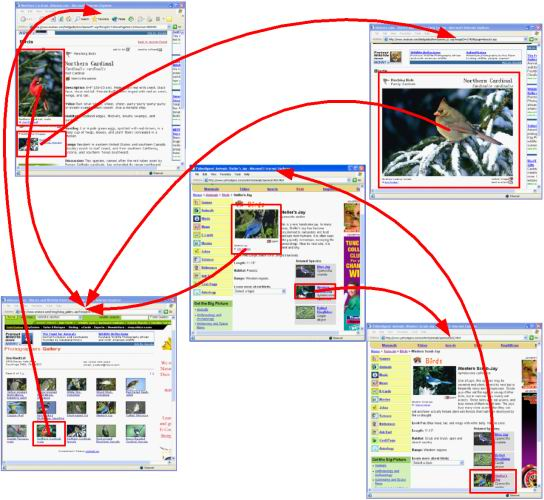
\includegraphics[width=0.5\textwidth]{example1_conn_graph.jpg}
    \caption{P\'aginas web y sus v\'inculos}
    \vspace{-24pt}
\end{wrapfigure}
\noindent

\par Un orden muy simple ser\'ia, por ejemplo, tomar el grado de entrada de cada
nodo\footnote{Es decir, la cantidad de ejes entrantes al nodo.}, u en palabras
de lo que representa el grafo, la cantidad de backlinks de una p\'agina y
ordenar en orden descendente por dicho valor. Pero esta soluci\'on presenta
un problema inmediato: todos los ''votos'' o ejes salientes tienen el mismo
peso, sin importar de qui\'en vienen. Si una p\'agina web tiene millones de
links, todos sus votos valen lo mismo que una p\'agina que s\'olo tiene diez. A
su vez, los votos de una p\'agina que no es votada por nadie valen lo mismo que
los de una p\'agina que es votada por todos los dem\'as.

\par Para solucionar, o al menos mitigar, este comportamiento, PageRank propone
cuantificar los ''votos'' seg\'un de quien vienen, y de su puntaje. Esto
inicialmente parecer\'ia un razonamiento circular ya que el puntaje de cada
p\'agina depender\'a del puntaje de las dem\'as, que a su vez dependen del
puntaje de esta p\'agina. Pero utilizando esta idea, con alguna modificaci\'on,
justamente se llegar\'a a un sistema de ecuaciones lineales, el cual permite
resolver justamente este tipo de c\'alculos donde hay muchas ecuaciones a ser
satisfechas que utilizan las mismas variables (en este caso, los puntajes de las
p\'aginas).

\par Volviendo a la cuantificaci\'on mencionada, la misma se basa en calcular el
puntaje de una p\'agina como la suma de los puntajes de las p\'aginas de sus
backlinks. Pero esto podr\'ia llevar a que una p\'agina con buen puntaje,
reparta infinitos votos (mediante la generaci\'on de links) de gran valor. Para
evitar esto se decide que el valor de los votos de una p\'agina sea distribuido
equitativamente entre todos sus votos. Formalizando un poco matem\'aticamente,
decimos que el puntaje $x_k$ de una p\'agina $k$ con el conjunto $L_k$ de
p\'aginas que tienen alg\'un link a $k$ se define como:

\begin{equation}\label{eq:calc_rank}
    x_k = \sum_{j\in L_k} \dfrac{x_j}{n_j} 
\end{equation}

donde $n_j$ es el grado de salida de $j$ (es decir, la cantida de links que
tiene la p\'agina $j$ o, lo que es equivalente, los ejes salientes del nodo
correspondiente a $j$).

\par En este modelo, se decide ignorar los links autoreferenciales (uno no puede
subir su ranking vot\'andose a si mismo), as\'i como tambi\'en considerar s\'olo
la conexidad entre dos nodos en lugar de considerar a todos los distintos links
que conectan en el mismo sentido el mismo par de p\'aginas (es decir, no
tenemos un multigrafo\footnote{Un grafo que permite tener varias aristas
conectando los mismos nodos (en el mismo sentido, en el caso de un grafo
dirigido).}).

\begin{wrapfigure}{l}{0.32\textwidth}
    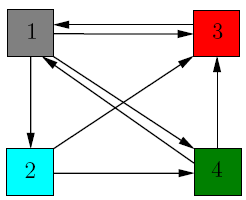
\includegraphics[width=0.3\textwidth]{example2_conn_graph.png}
    \caption{Grafo de conexidad}
    \label{fig:graph_conn}
    \vspace{-24pt}
\end{wrapfigure}
\noindent

\par Observemos en la figura \ref{fig:graph_conn} un ejemplo de un grafo de
conexidad entre las p\'aginas $1, 2, 3$ y $4$:

\par Aplicando la ecuaci\'on \ref{eq:calc_rank} en este ejemplo, obtenemos que
el siguiente sistema de ecuaciones:

\begin{equation}
    \begin{cases}
        n_1 = 3\\
        n_2 = 2\\
        n_3 = 1\\
        n_4 = 2
    \end{cases}
    \implies
    \begin{cases}
        x_1 = x_3/1 + x_4/2\\
        x_2 = x_1/3\\
        x_3 = x_1/3 + x_2/2\\
        x_4 = x_1/3 + x_2/2
    \end{cases}
\end{equation}

\par Y como ya se ha visto a lo largo de la materia, este sistema de ecuaciones
es expresable como un sistema $Ax = x$ para $A\in\real^{4\times4}$ y
$x\in\real^4 $ (pues $\overrightarrow{x}$ es tanto el vector de coeficientes
como el vector resultado):

\begin{equation}
    \underbrace{
        \begin{bmatrix}
                0& 0& 1& \frac{1}{2}\\[-0.65em]
                \frac{1}{3}& 0& 0& 0\\[-0.65em]
                \frac{1}{3}& \frac{1}{2}& 0& \frac{1}{2}\\[-0.65em]
                \frac{1}{3}& \frac{1}{2}& 0& 0
        \end{bmatrix}
    }_A
    \underbrace{
        \begin{bmatrix}
            x_1\\[-0.65em]
            x_2\\[-0.65em]
            x_3\\[-0.65em]
            x_4
        \end{bmatrix}
    }_x
    =
    \underbrace{
        \begin{bmatrix}
            x_1\\[-0.65em]
            x_2\\[-0.65em]
            x_3\\[-0.65em]
            x_4
        \end{bmatrix}
    }_x
\end{equation}

\par Esta matriz $A$ obtenida, si se observa bien, es lo que podr\'iamos llamar
una matriz de conexidad pesada. Esto se nota al caracterizar el valor de cada
coordenada de la matriz:

\begin{equation}
    a_{ij} =
    \begin{cases}
        0       &\text{si $j$ no tiene links a $i$}\\
        1/n_j   &\text{si $j$ tiene links a $i$}
    \end{cases}
\end{equation}

\par Entonces vemos que la matriz tiene valores no nulos siempre que haya un
link de $j$ a $i$, y en tal caso el valor de la matriz ser\'a algo similar a
repartir el ''\'unico'' voto del nodo $j$ entre todas sus conexiones/ejes
salientes ($n_j$)\footnote{Decimos ''\'unico voto'' pues en $A$ no est\'an los
rankings de las p\'aginas (los $x_k$). Esto se puede entender como que todas las
p\'aginas tienen el mismo poder de voto (igual a 1) pero lo reparte de manera
equitativa entre todas las p\'aginas a las cuales se v\'incula.}.
\medskip

\par Partimos entonces de un modelo basado en digrafos\footnote{Grafos
dirigidos.} y una expresi\'on matem\'atica para el c\'alculo del puntaje de cada
nodo, y llegamos al problema de resolver un sistema del tipo $Ax = x$, que es
equivalente a resolver $Ax = \lambda x$ con $\lambda = 1$. Y esto \'ultimo no es
otra cosa que calcular el autovector asociado al autovalor $1$ de la matriz $A$
~\cite[p.~443]{Burden2010}.

\par Claramente, antes de comenzar a resolver este problema hay que plantearse
si el mismo tiene soluci\'on. En este caso, deber\'iamos poder asegurar la
existencia de un autovalor 1. Por suerte para el modelo, se puede asegurar que
existir\'a dicho autovalor si la matriz es \emph{estoc\'astica por
columnas}\footnote{Se dice que una matriz es estoc\'astica por columnas si todos
sus valores son no negativos y la suma de los valores de cualquier columna es
igual a 1.}~\cite[p.572]{Bryan2006}, con lo cual para asegurar que existir\'a el
$x$ buscado, podr\'iamos tratar de ver si $A$ es estoc\'astica por
columnas\footnote{Las matrices estoc\'asticas por columnas son tambi\'en
llamadas en determinada bibliograf\'ia como matrices de \emph{Markov}.}.

\par En \cite[p.572]{Bryan2006} se demuestra que la matriz $A$ es estoc\'astica
por columnas si el grafo asociado est\'a libre de \emph{dangling nodes}, o
nodos con grado de salida 0 (es decir, p\'aginas web sin links). Matricialmente
hablando, esto ser\'ia una columna de A con ceros \'unicamente. As\'i pues,
encontramos una primera cosa que modelo debe solucionar para asegurar la
existencia del autovalor 1.

\par Otro problema que surge es la posibilidad de que el autovalor 1 de esta
matriz (suponiendo que se aseguro la no existencia de los dangling nodes) tenga
multiplicidad mayor a 1. Es decir, que tengamos m\'ultiples soluciones para
nuestro modelo (m\'ultiples posibles rankings). Claramente esto es algo no
deseado, ya que no tenemos un patr\'on para decidir que ranking es el correcto
en caso de tener varios. As\'i pues, aqu\'i encontramos otro inconveniente a
solucionar: la existencia de rankings m\'ultiples.


\subsubsection{Dangling Nodes y Rankings M\'ultiples}

\par Hasta ahora, hemos observado al modelo para puntuar a las p\'aginas basados
\'unicamente en los links entre las mismas, sin tomar en cuenta el
comportamiento de los usuarios navegando en las p\'aginas. PageRank, en su
primera versi\'on, propone que todo usuario siempre puede decidir ir a la barra
de direcci\'on e ir a cualquier p\'agina con la misma probabilidad. Obviamente,
esto \'ultimo no es del todo fino y puede ser mejorado, es mucho m\'as probable
que usuario escriba la direcci\'on de un buscador web, o de alguna p\'agina
relacionada con el mismo \'ambito de la p\'agina actual en la que se
encuentra~\footnote{Cosas que \emph{Google} seguramente comenz\'o a tomar en
cuenta en siguientes versiones de su buscador.}. A\'un as\'i, dado el contexto
did\'actico de este trabajo, utilizaremos esta versi\'on en la cual se asume que
el navegador elige con la misma probabilidad cualquiera de las p\'aginas a las
cuales ''saltar'' mediante la barra de direcciones (tal como lo hicieron Bryan y
Page en 1998).  A este proceso de ''saltar'' a cualquier otra p\'agina/nodo del
grafo se lo denomina \emph{teletransportaci\'on}.

\par Volviendo a nuestra matriz $A$, se utiliza el concepto de teletransportaci\'on
de manera concistente con el modelo, de manera de convertir a $A$ en una matriz
sin dangling nodes y que represente a un grafo conexo\footnote{Cosa que en la
realidad no necesariamente pasa. Como ejemplo, alcanza conque exista una
p\'agina web que no sea referenciada ni que referencie a otros sitios web. O
alg\'un tipo de documento web, como un \emph{pdf}}, o equivalentemente,
convertirla a una matriz de Markov irreducible. Luego la teor\'ia de cadenas de
Markov nos asegurar\'a la existencia del autovalor 1 (pues una matriz de Markov
es estoc\'astica por columnas por definici\'on, y ya hemos comentado hace
algunos p\'arrafos que en tal caso existe el autovalor 1) y la unicidad del
autovector asociado (nuestro $\overrightarrow{x}$).

\par La idea intutiva planteada por Brian y Page fue la del \textbf{navegante
aleatorio}. B\'asicamente plantean que existe un usuario (o navegante) que va
''viajando'' entre los links de la estructura del grafo/web. Es decir, cuando
llega a una p\'agina con muchos links, elige uno aleatoriamente y llega a una
nueva p\'agina. Este proceso sigue indefinidamente. Pensando en el infinito, la
proporci\'on del tiempo que este navegante pasa en una p\'agina dada ser\'ia la
medida de la importancia relativa de dicho sitio (respecto de las dem\'as
p\'aginas). A mayor proporci\'on, mayor importancia, por lo tanto, deber\'ia
tener mayor puntaje. Entonces las cuestiones de los dangling nodes aqu\'i se
notan como un problema evidente, ya que una vez que llega a uno de ellos, el
navegante no puede continuar. Aqu\'i se utiliz\'o la teletransportaci\'on para
solucionar este inconveniente.

\par Se realiza entonces un \textbf{ajuste estoc\'astico} sobre $A$, donde todas
las columnas $\overrightarrow{0}$ son reemplazadas por columnas
$(\rfrac{1}{n})e$, para $e = \overrightarrow{1}$ y $n$ la cantidad de
nodos/p\'aginas. De esta manera la matriz $A$ se vuelve estoc\'astica por
columnas/matriz de Markov, ya que las columnas correspondientes a los dangling
nodes ahora tienen $n$ valores de $1/n$, y su sumatoria es $1$ trivialmente.
As\'i pues, se resolvi\'o el inconveniente de los dangling nodes y se
convirti\'o a $A$ en una matriz de Markov, para la cual ya se asegur\'o la
existencia del autovalor 1.

\par Matricialmente hablando, tendr\'iamos que:

\begin{equation}
    S = A + \left(\dfrac{1}{n}e\right)a^T \quad\quad\quad
        \text{Donde: } a_i =
        \begin{cases}
            1 &\text{si el nodo $i$ es un dangling node}\\
            0 &\text{caso contrario}
        \end{cases}
\end{equation}
\medskip

\par Tomemos un ejemplo para que se vea precisamente como esto elimina los
dangling nodes de un grafo. En la figura \ref{fig:dang_node} tenemos el mismo
ejemplo anterior, pero habiendo eliminado el link de $3$ a $1$, convirti\'endo
el nodo $3$ en un dangling node.

\begin{wrapfigure}{l}{0.32\textwidth}
    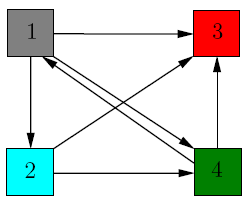
\includegraphics[width=0.3\textwidth]{example3_dangling_node.png}
    \caption{Dangling Nodes}
    \label{fig:dang_node}
    \vspace{-24pt}
\end{wrapfigure}
\noindent

\begin{equation*}
    S = \underbrace{
        \begin{bmatrix}
                0& 0& 0& \frac{1}{2}\\[-0.65em]
                \frac{1}{3}& 0& 0& 0\\[-0.65em]
                \frac{1}{3}& \frac{1}{2}& 0& \frac{1}{2}\\[-0.65em]
                \frac{1}{3}& \frac{1}{2}& 0& 0
        \end{bmatrix}
    }_A + \underbrace{
        \begin{bmatrix}
            \frac{1}{4}\\[-0.65em]
            \frac{1}{4}\\[-0.65em]
            \frac{1}{4}\\[-0.65em]
            \frac{1}{4}
        \end{bmatrix}
    }_{\dfrac{1}{n}e} \underbrace{
        \begin{bmatrix}
            0 & 0 & 1 & 0
        \end{bmatrix}
    }_{a^T}
    =
    \begin{bmatrix}
            0& 0& 0& \frac{1}{2}\\[-0.65em]
            \frac{1}{3}& 0& 0& 0\\[-0.65em]
            \frac{1}{3}& \frac{1}{2}& 0& \frac{1}{2}\\[-0.65em]
            \frac{1}{3}& \frac{1}{2}& 0& 0
    \end{bmatrix} %+
    \begin{bmatrix}
        0&0&\frac{1}{4}&0\\[-0.65em]
        0&0&\frac{1}{4}&0\\[-0.65em]
        0&0&\frac{1}{4}&0\\[-0.65em]
        0&0&\frac{1}{4}&0
    \end{bmatrix}
\end{equation*}
\begin{equation}
    S =\begin{bmatrix}
        0& 0& \frac{1}{4}& \frac{1}{2}\\[-0.65em]
        \frac{1}{3}& 0& \frac{1}{4}& 0\\[-0.65em]
        \frac{1}{3}& \frac{1}{2}& \frac{1}{4}& \frac{1}{2}\\[-0.65em]
        \frac{1}{3}& \frac{1}{2}& \frac{1}{4}& 0
    \end{bmatrix} %+
\end{equation}


%-------------------------------------------------------------------------------
\subsection{Adaptaci\'on a Eventos Deportivos}


%-------------------------------------------------------------------------------
